\begin{frame}{What is a cloud?}
	\begin{center}
		\begin{figure}
			\centering
			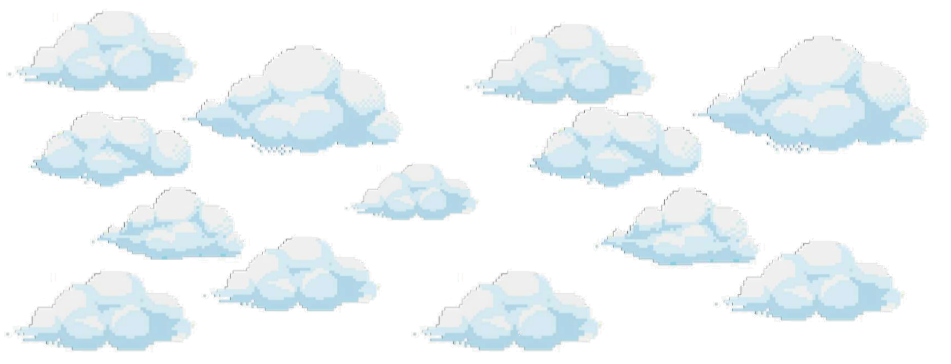
\includegraphics[width=0.8\linewidth]{images/intro_fig00_0.png}
			\label{fig:introfig01}
	\end{figure}
	\vspace{20px}
	\textbf{A cloud is a mass of water drops or ice crystals suspended in the atmosphere.}	
	\end{center}
\end{frame}


\begin{frame}{What is a cloud?}
	\begin{center}
		\begin{figure}
			\centering
			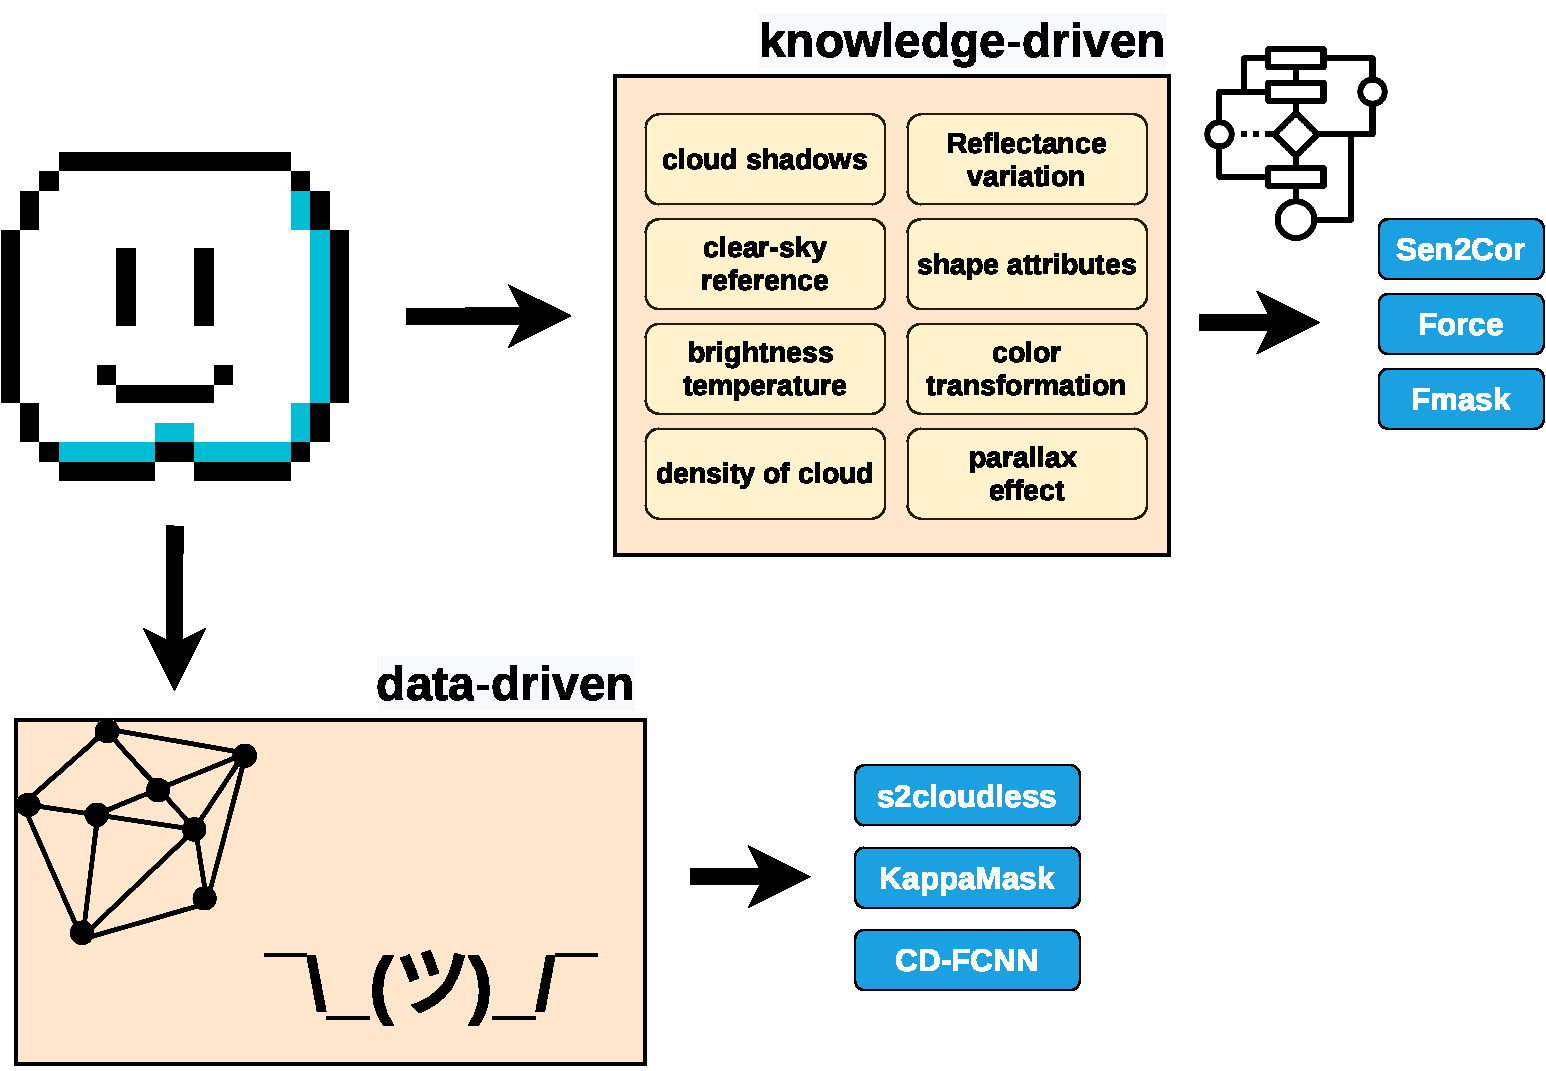
\includegraphics[width=0.85\linewidth]{images/intro_what_is_a_cloud.pdf}
			\label{fig:introfig01}
		\end{figure}
	\end{center}
\end{frame}


\begin{frame}{Context - I}
	\begin{center}
		\begin{figure}
			\centering
			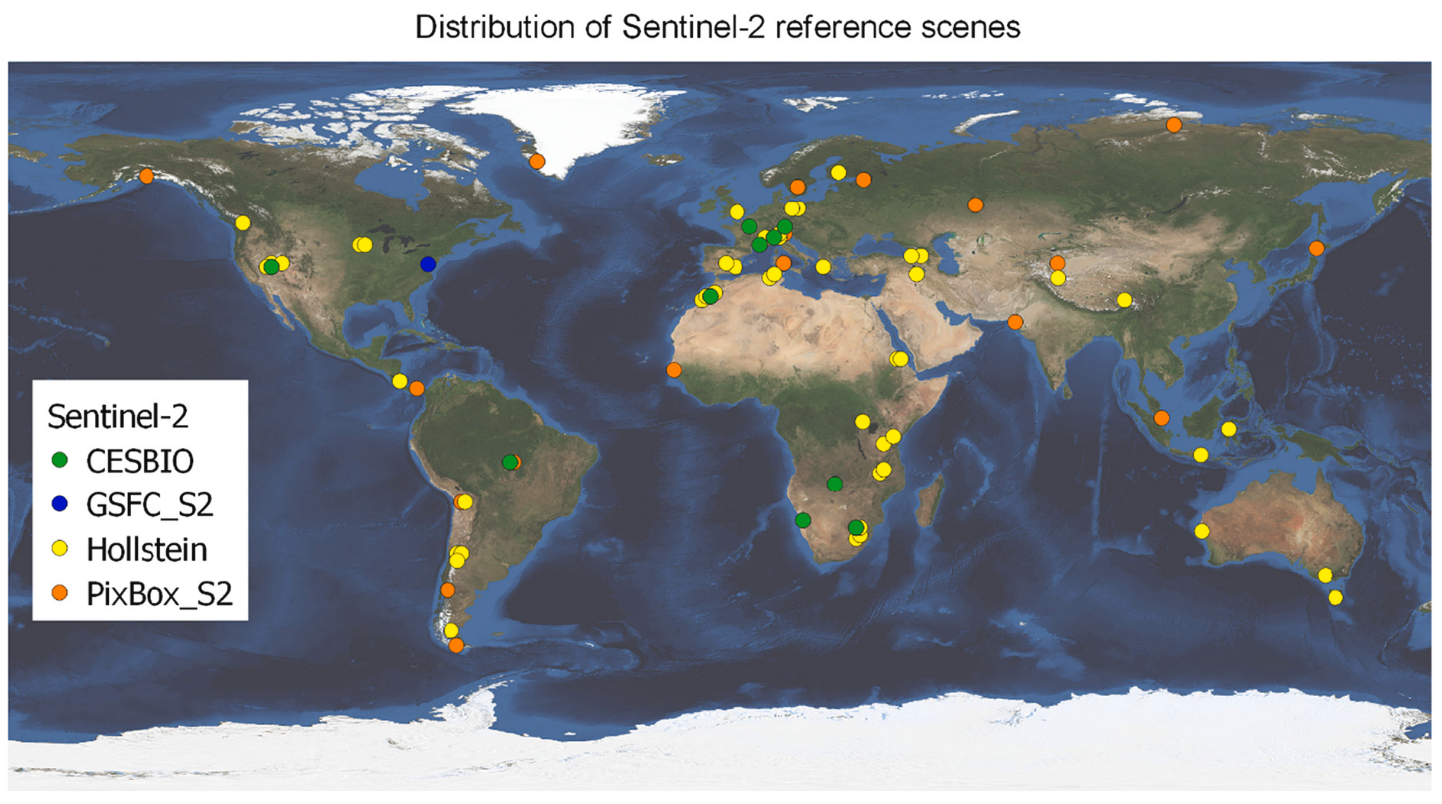
\includegraphics[width=0.85\linewidth]{images/intro_fig01.png}
			\caption[fig:introfig01]{Geographical distribution reference cloud detection datasets for Sentinel-2 (Skakun et al. 2022).}
			\label{fig:introfig01}
		\end{figure}
	\end{center}
\end{frame}


\begin{frame}{Context - II}
	\begin{columns}
		\begin{column}{0.5\textwidth}
			\begin{figure}
				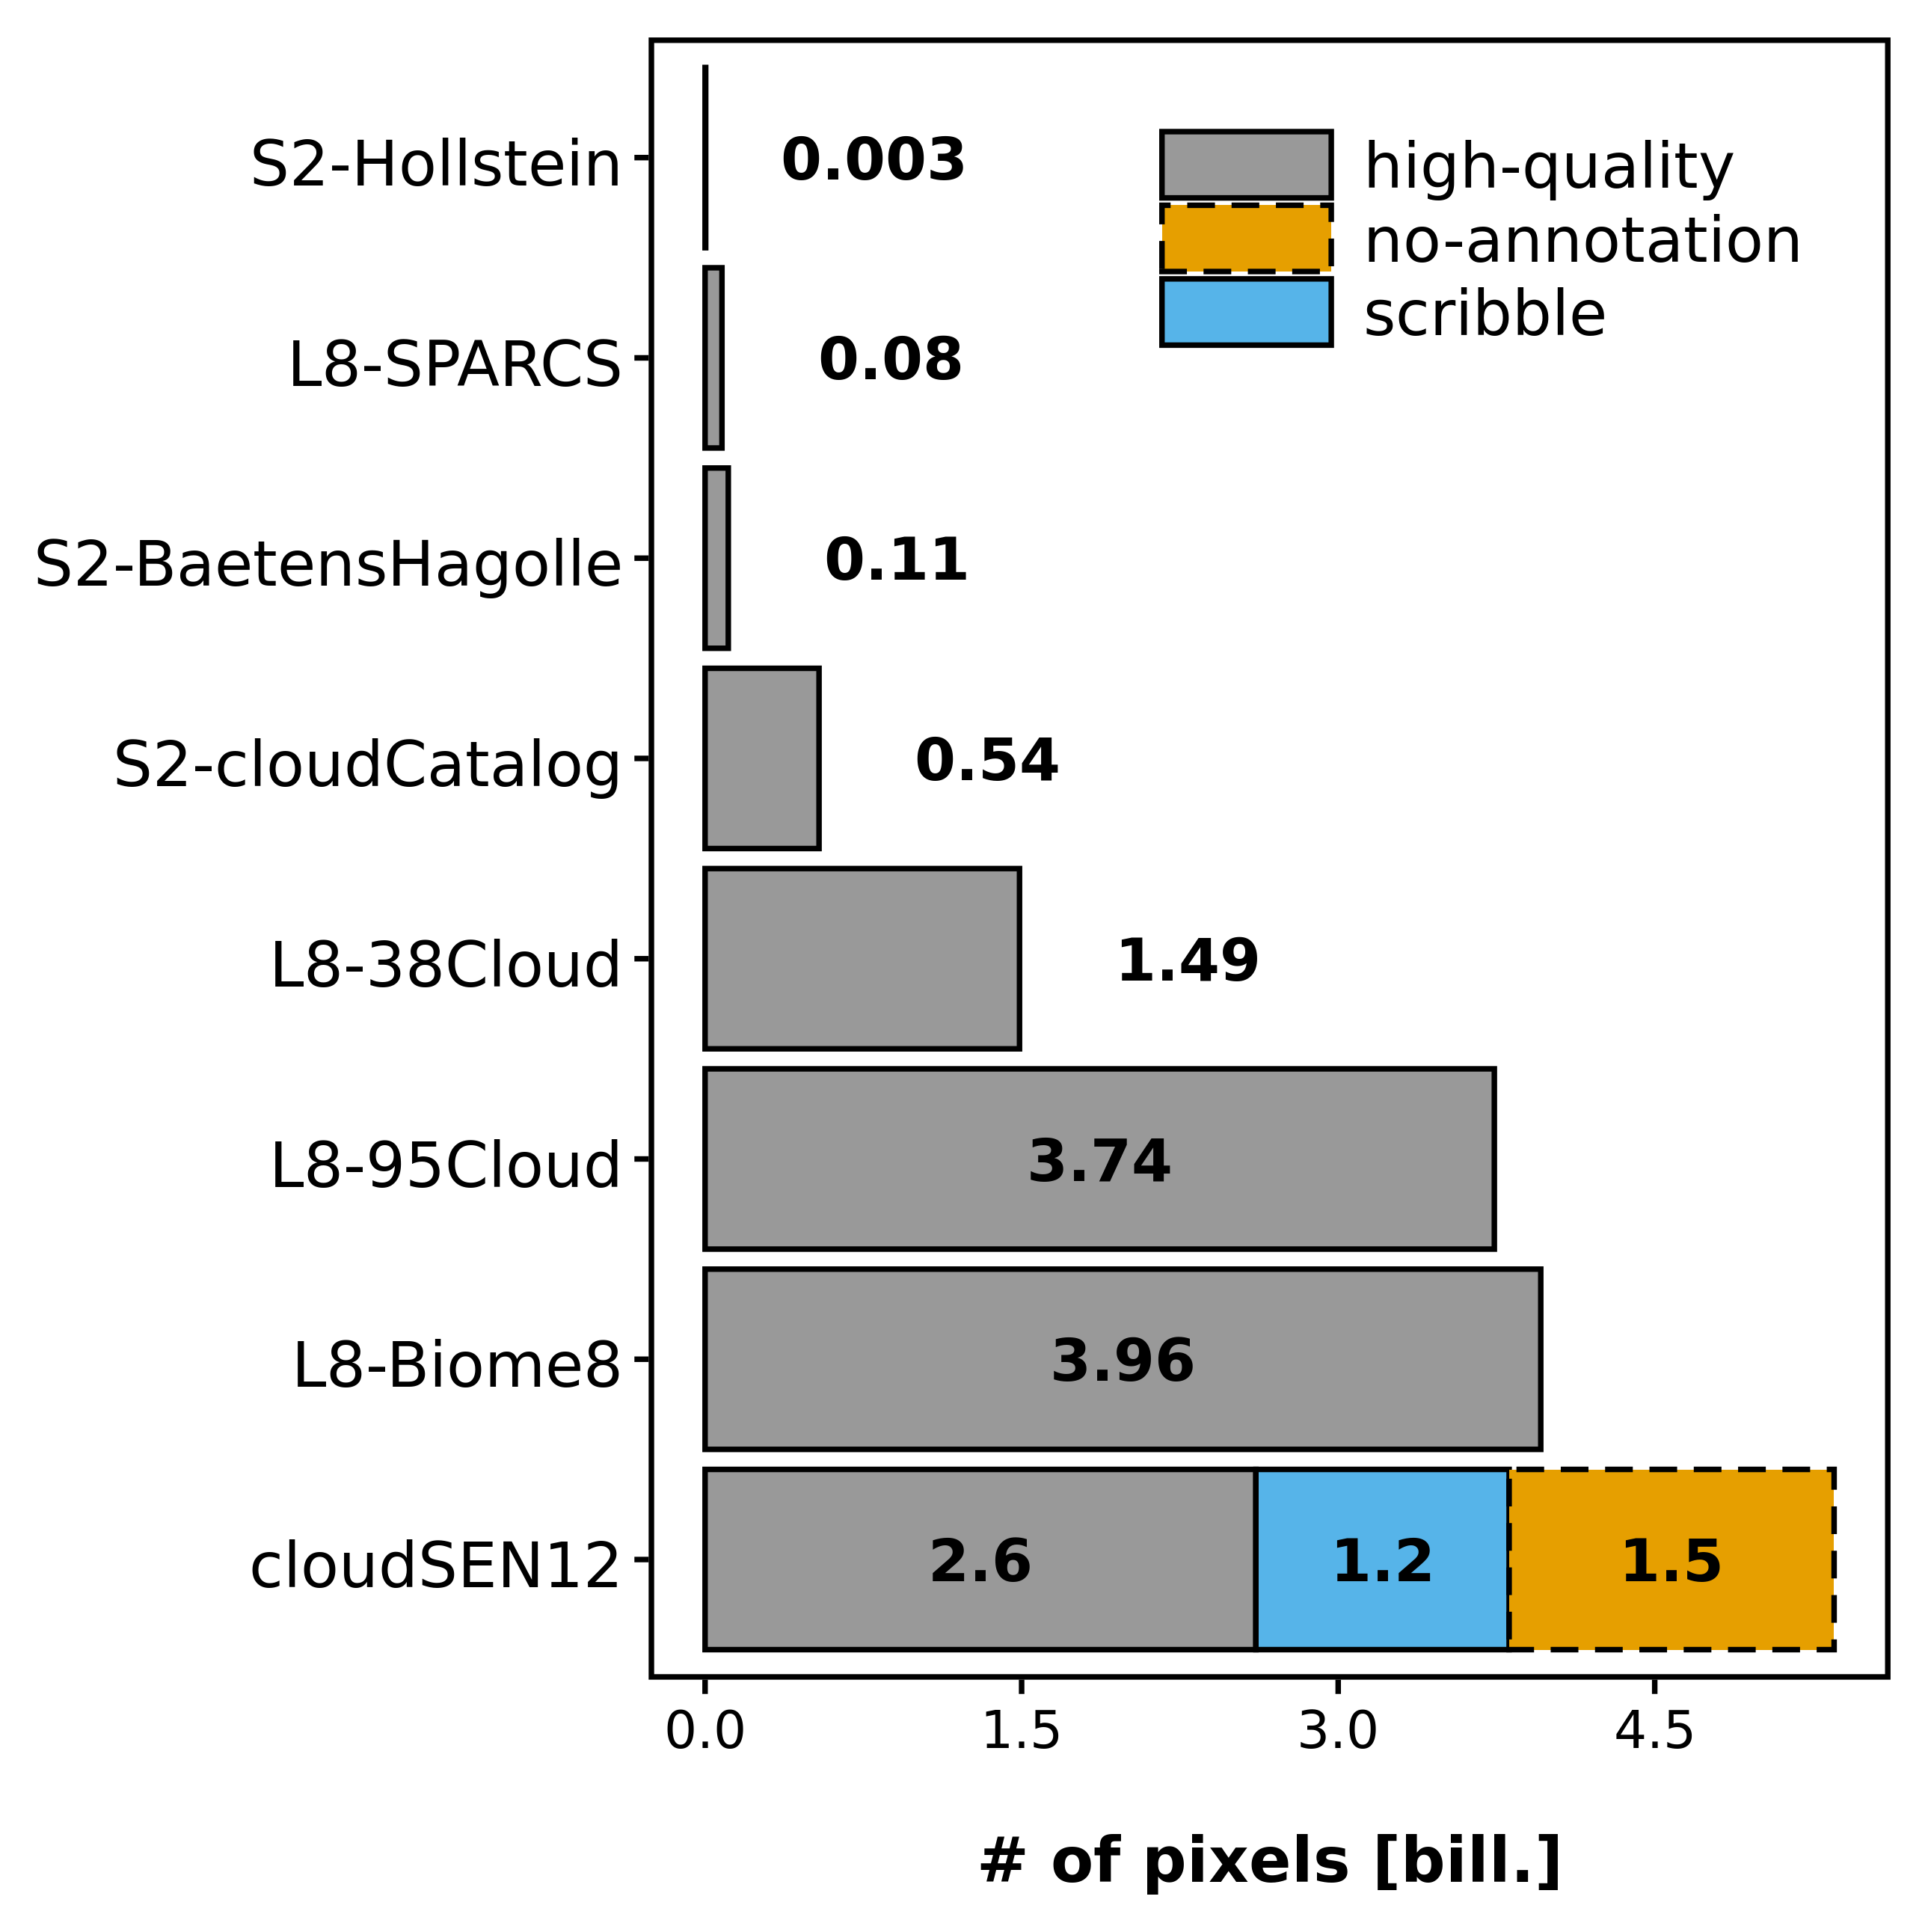
\includegraphics[width=\textwidth]{images/intro_fig02.png}
				\label{fig:introfig02}
			\end{figure}	
		\end{column}
		\begin{column}{0.5\textwidth}
			\begin{itemize}[<+->]
				\item Cloud labels created by human photo-interpretation, active learning and ground-based camaras.
				\item \textbf{No temporal features}.
				\item High class imbalance.
				\item Created by \textbf{\textit{closed science practices}}.
				\item \textbf{The quality of some datasets is poor.}
			\end{itemize}
		\end{column}
	\end{columns}
\end{frame}


\begin{frame}{CloudSEN12 - I}
	\begin{center}
		\begin{figure}
		\animategraphics[width=0.55\linewidth,loop,autoplay]{10}{images/gif01/frame-}{0}{6}		
		\end{figure}		
	\textcolor{blue}{\href{https://cloudsen12.github.io/}{https://cloudsen12.github.io/}}
	\end{center}
\end{frame}


\begin{frame}{Context - II}
	\begin{center}
		\begin{figure}
			\centering
			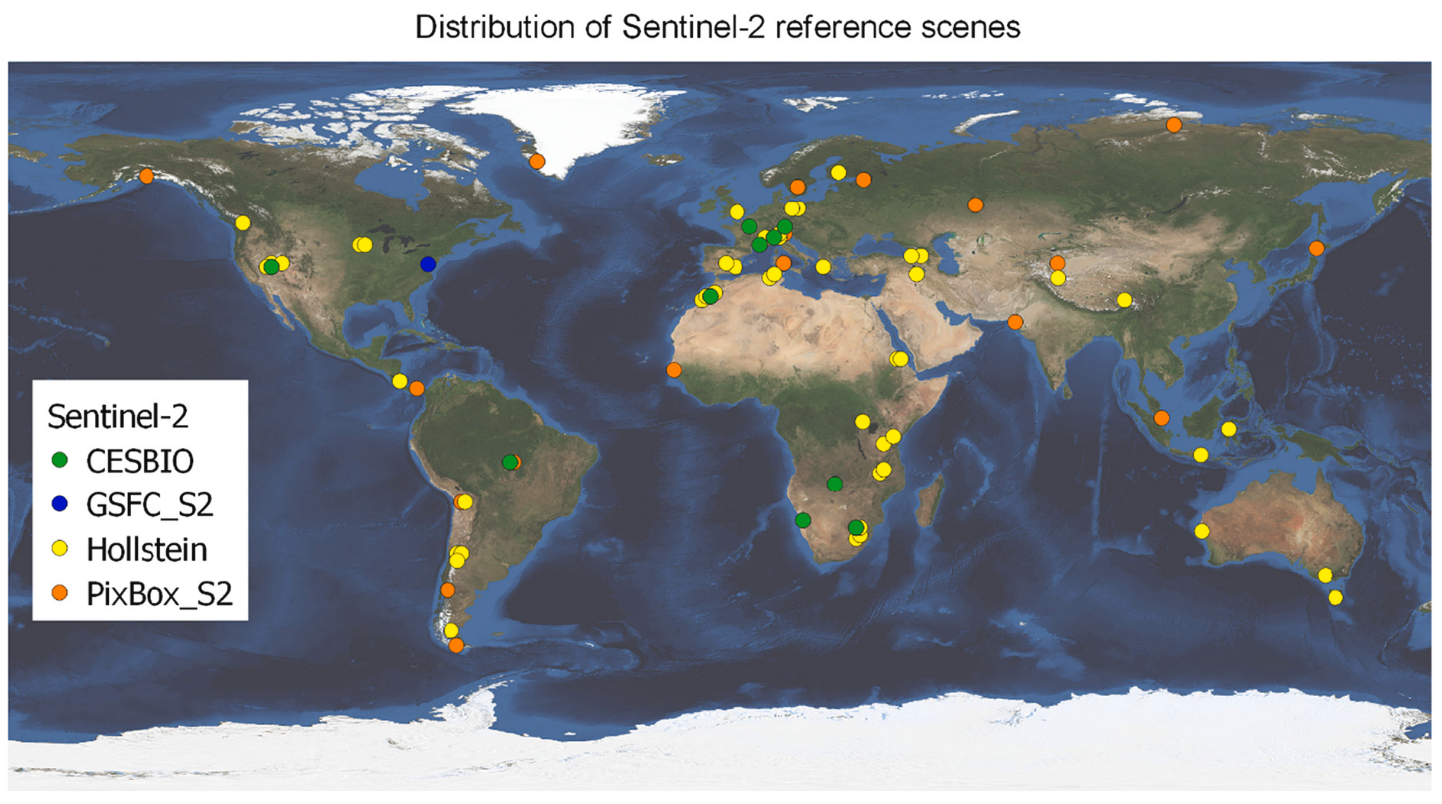
\includegraphics[width=0.85\linewidth]{images/intro_fig01.png}
			\caption[fig:introfig01]{Geographical distribution reference cloud detection datasets for Sentinel-2 (Skakun et al. 2022).}
			\label{fig:introfig01}
		\end{figure}
	\end{center}
\end{frame}

\begin{frame}{CloudSEN12 - II}
	\begin{center}
		\begin{figure}
			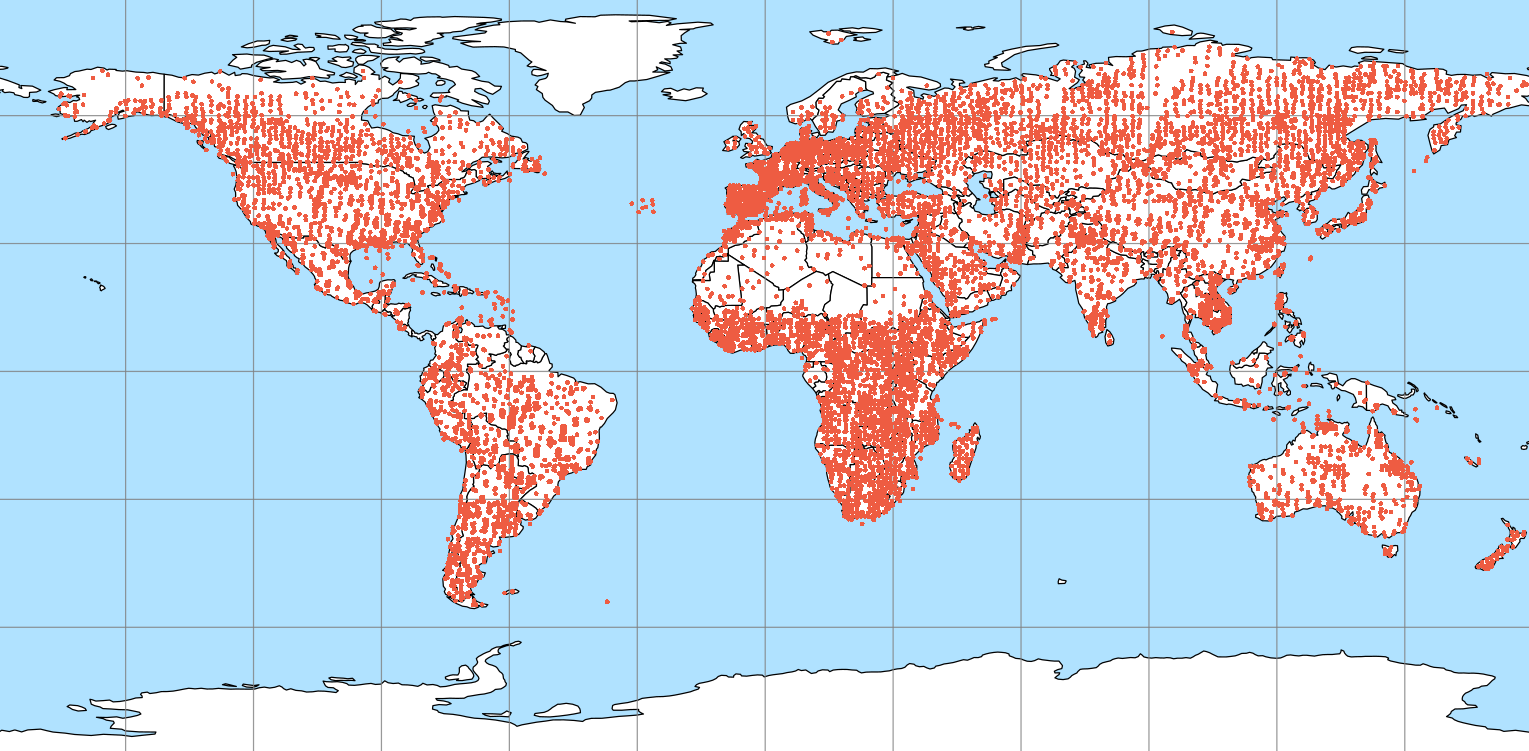
\includegraphics[width=0.85\linewidth]{images/intro_fig04.png}
			\caption[fig:introfig04]{CloudSEN12 spatial distribution}
		\end{figure}
	\end{center}
\end{frame}
